\documentclass{uiucecethesis09}
\usepackage{mythesis}

\begin{document}
\chapter{Background}
  \label{chap:background}

  To understand the techniques used in this project, it is necessary to 
  understand certain background material. Namely, what microphone arrays are and 
  what can be done with them. The techniques covered in this chapter will 
  heavily influence the material in later chapters and provide a foundation for 
  the work in the rest of the project.

  \section{Microphone Arrays}

    \subsection{Properties}
      In this project, we will use fixed microphone arrays, which are comprised 
      of a set of $\nmics$ microphones arranged in some fixed geometry. 

      A popular example of a microphone array is the equally spaced linear 
      array, which consists of $\nmics$ microphones in a line with a distance 
      $d$ between each consecutive microphone. An illustration of this is given 
      in \figref{fig:lin_mic_array}, and an example of such a system in 
      \figref{fig:ps3_eye}.  The popularity of this configuration comes from the 
      ease with which analysis can be performed due to the simplicity of the 
      geometry.  However, several other geometries are possible. A circular 
      microphone array is shown in \figref{fig:circle_array} and a three 
      dimensional 'cone' geometry is shown in \figref{fig:microcone}. In this 
      project we will make use of the PS3 Eye (shown in \figref{fig:ps3_eye}) 
      and the Dev Audio Microcone (shown in \figref{fig:microcone}) for our 
      experiments.

      % Linear Microphone Array Figure
      \begin{figure}[bottom]
        \begin{center}
          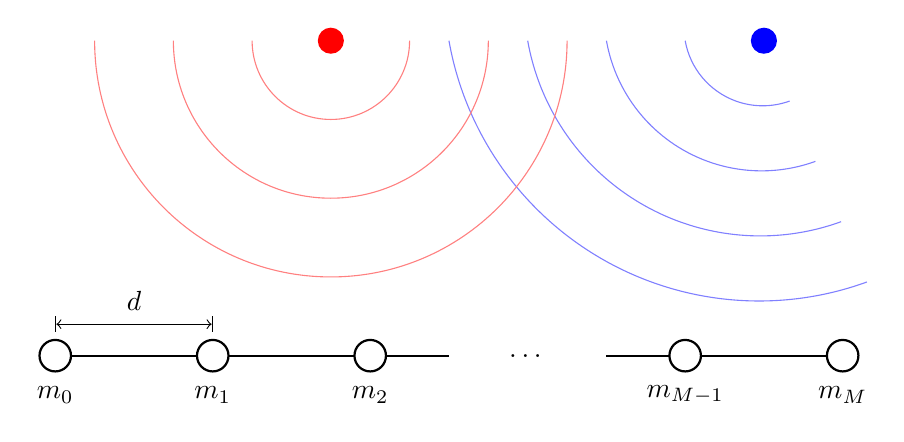
\begin{tikzpicture}
  [mic/.style={shape=circle, black, fill=white, thick, minimum size=4mm}]
  % Setup constants
  \def\miclineoffset{.4}
  \pgfmathsetmacro{\doffset}{\miclineoffset+.3}
  \pgfmathsetmacro{\miclabeloffset}{-.5}
  % Draw the lines on which the microphones will lie
  \draw [thick] (0,0) -- (5,0);
  \draw [thick] (7,0) -- (10,0);
  % Draw the first three mics in the group
  \draw [|<->|] (0,\miclineoffset) -- (2, \miclineoffset);
  \foreach \x in {0, 1, 2} {
    \node at (2*\x, 0) [mic, draw] {};
    \node at (2*\x, \miclabeloffset) {$m_{\x}$};
  }
  % Separator between sets of nodes
  \node at (6, 0) {\ldots};
  % Last few nodes that will be indexed from the end (M)
  \node at (8, 0) [mic, draw] {};
  \node at (8, \miclabeloffset) {$m_{M-1}$};
  \node at (10, 0) [mic, draw] {};
  \node at (10, \miclabeloffset) {$m_{M}$};
  \node at (1, \doffset) [] {$d$};

  % Draw arcs for sound waves
  \node[circle, fill=blue] at (9, 4) {};
  \foreach \rad in {1, 2, 3, 4} {
    \draw[blue!50] (9-\rad, 4) arc [start angle=190, end angle=290, 
    radius=\rad];
  }
  \node[circle, fill=red] at (3.5, 4) {};
  \foreach \rad in {1, 2, 3} {
    \draw[red!50] (3.5-\rad, 4) arc [start angle=180, end angle=360, 
    radius=\rad];
  }
\end{tikzpicture}

        \end{center}
        \caption{Linear microphone array configuration. Each microphone $m_\micidx$ 
        lies on a line and is separated from adjacent microphones by a distance 
      $d$.  There are two example sound sources.}
        \label{fig:lin_mic_array}
      \end{figure}

      % Examples of different microphone arrays
      \begin{figure}[b]
        \centering
        \begin{subfigure}[b]{.45\textwidth}
          \includegraphics[width=\textwidth]{\thesisdir/background/figures/ps3_eye.jpg}
          \caption{PS3 Eye. Contains 4-microphone equidistance linear array}
          \label{fig:ps3_eye}
        \end{subfigure}
        \quad
        \begin{subfigure}[b]{.45\textwidth}
          \includegraphics[width=\textwidth]{\thesisdir/background/figures/circle_array.png}
          \caption{ An eight-element circular microphone array 
            \cite{tashev2009sound}}
          \label{fig:circle_array}
        \end{subfigure}
        
        \begin{subfigure}[b]{\textwidth}
          \centering
          \includegraphics[width=.5\textwidth]{\thesisdir/background/figures/microcone.png}
          \caption{ The Dev Audio Microcone. This microphone array has six 
          microphones on the faces of a hexagonal base and one microphone at the 
        tip of the cone.}
          \label{fig:microcone}
        \end{subfigure}
        \caption{Microphone array examples}
        \label{fig:mic_array_examples}
      \end{figure}

      It may not be immediately apparent how a microphone array can provide any 
      advantage for processing signals. At each microphone we should expect to 
      hear the same signal with some delay, so how does this provide any 
      advantage?  
      
      One answer to this is that the signals will not be exactly the same at 
      each microphone; in fact, they will usually be corrupted by some noise in 
      the environment. The redundancy of the recordings can then be used to help 
      deduce what part of the signal is interesting, and what part of the signal 
      is noise. This is largely the focus of beamforming techniques and will be 
      reviewed in a later section
      
      However, even if the signals recorded at each microphone are just shifted 
      versions of the exact same source signal, there is still a gain to be had 
      from using multiple microphones. This is because by using a fixed 
      microphone array, one has infused the samples with spatial information -- 
      the information inherent in the spatial geometry of the array. In fact, 
      because of this it is possible to find the directivity of an array by 
      using the spatial Fourier transform \cite{benesty2010microphone}. It is 
      possible to use this property to infer spatial information about the 
      source.

    \subsection{Setup}
      \label{sec:setup}
      Consider a microphone array composed of $\nmics$ microphones with 
      microphone $\micidx$ located at position $\vect{\micpos}_\micidx$. Take the position 
      matrix $\mat{P}$ to be the matrix whose columns are composed of the 
      positions of the microphones:

      % Draw Position matrix
      \begin{equation} \label{eq:pos_mat}
        \mat{\posmat} =
          \begin{bmatrix} | & | && | \\
            \micpos_1 & \micpos_2 & \ldots & \micpos_\nmics \\
              | & | && |
          \end{bmatrix}
      \end{equation}

      Assume that there is some source signal $\srcsig(t)$ emanating from a 
      point source at position $\vect{\srcpos}$. Furthermore, assume that 
      $\vect{\srcpos}$ is far enough from each microphone that the far field 
      assumption holds. That is, the sound wave can be viewed as a plane wave 
      associating each microphone from the same direction. See TODOFIGURE for an 
      illustration. 
      
      Now select one of the microphones to be used as reference for the others.  
      We choose the first microphone.  It is possible to calculate the amount of 
      time it takes the sound signal to reach the reference microphone
      % Mic delays
      \begin{equation} \label{eq:ref_delay} \refdelay = \frac{\norm{\srcpos - 
        \micpos_1}}{\speedsound} \end{equation}
      where $\speedsound$ is the speed of sound.  In addition to this, we can 
      calculate the amount of time it takes for the sound to travel between the 
      reference microphone and any other microphone.  To do this we make use of 
      the far field model \cite{dudgeon1977fundamentals}.  Assume the sound wave 
      is a plane wave and $\srcdir$ is a unit vector pointing in the direction 
      of the sound source as viewed by the center of the microphone array. We 
      then have that
      \begin{equation} \label{eq:TDOA} \micdelay_\micidx = \frac{\left(\micpos_1 
        - \micpos_\micidx\right) \cdot \srcdir}{\speedsound} \end{equation}
      where $\micdelay_\micidx$ is the delay between the arrival of the signal 
      at microphone 1 and the arrival of the signal at microphone $\micidx$.  
      This is known as a time difference of arrival (TDOA).  This gives 
      \begin{align} \label{eq:mic_signal}
        \micrec_\micidx\oftime &= \atten_\micidx\srcsig\of{\sigtime - \refdelay - 
        \micdelay_\micidx} + \micnoise_\micidx\oftime\\
        &= \micsig_\micidx\oftime + \micnoise_\micidx\oftime
      \end{align}
      where $\micrec_\micidx\oftime$ is the signal recorded at microphone $\micidx$, 
      $\srcsig\oftime$ is the unknown source signal, $\alpha_\micidx$ are the 
      attenuation factors, and $\micnoise_\micidx\oftime$ are the additive noise heard 
      at each microphone.

      From this equation we see that if we assume all $\atten_\micidx$ are equal 
      we have
      \begin{equation} \label{eq:sig_shift} \micsig_\micidx\oftime = 
        \micsig_1\of{\sigtime - \micdelay_\micidx} \end{equation}
      which reaffirms the intuitive notion that the signal recorded at each 
      microphone will be just a shifted (and likely distorted) version of the 
      signal occurring at the reference microphone.
      
  \section{Beamforming}

    \subsection{Array Directivity}
      In \eqref{eq:sig_shift} we saw that each signal is just a shifted version 
      of the signal at the first microphone. In turn if we want to align the 
      signals we need only reverse such a shift. To do so we transfer our focus 
      to the frequency domain.
      The frequency domain equivalent of \eqref{eq:sig_shift} gives the 
      following
      \begin{equation} \label{eq:freq_shift} \Micsig_\micidx\offreq = 
        \Micsig_1\offreq e^{-j2\pi\freq\micdelay_\micidx}
        \end{equation}
      Now take the vector
      \begin{equation} \label{eq:steering_vec}
        \steer\of{\dir, \freq} =
        \begin{bmatrix} e^{j2\pi\freq\micdelay_1\of{\dir}} & 
          e^{j2\pi\freq\micdelay_2\of{\dir}} & \cdots & 
          e^{j2\pi\freq\micdelay_\nmics\of{\dir}}
        \end{bmatrix}\trans
      \end{equation}
      which can be seen to contain the opposite shifts for each microphone. Note 
      that here $\micdelay_\micidx$ has been written as a function of $\dir$ to 
      emphasize the dependence of the delays on a given steering direction. Now 
      if we look at the vector
      \begin{equation}
        \Micsig\offreq = \begin{bmatrix} \Micsig_1\offreq & \Micsig_2\offreq 
          & \cdots & \Micsig_\nmics\offreq \end{bmatrix}\trans
      \end{equation}
      we see that the vector product
      \begin{align}
        \steer\of{\dir, \freq}\trans \Micsig\offreq &= 
        \sum\limits_{\micidx=1}^{\nmics} \Micsig_\micidx\offreq 
        e^{j2\pi\freq\micdelay_\micidx\of{\dir}} \\
        &= \sum\limits_{\micidx=1}^{\nmics} \Micsig_\micidx\offreq 
        e^{j2\pi\freq\frac{\left(\micpos_1 - \micpos_\micidx\right) \cdot 
        \dir}{\speedsound}} \\
        &= \sum\limits_{\micidx=1}^{\nmics} \Micsig_\micidx\offreq 
        e^{-j2\pi\freq\frac{\left(\micpos_\micidx - \micpos_1\right) \cdot 
        \dir}{\speedsound}} \\
        &= \sum\limits_{\micidx=1}^{\nmics} \Micsig_\micidx\offreq 
        e^{-j2\pi\vect{\xi} \cdot \left(\micpos_\micidx - \micpos_1\right)}
      \end{align}
      equates to a spatial Fourier Transform, where
      \begin{equation} \vect{\xi} = \frac{\freq\dir}{\speedsound} \end{equation}
      is the spatial frequency vector. Just as a spectral Fourier Transform can 
      be interpreted as determining the energies in each constituent frequency 
      of a signal, this spatial Fourier Transform can be viewed as determining 
      the energies in each constituent direction of the signal, given a specific 
      frequency of the signal. This makes sense as here we sample the signal 
      across space where as in the spectral version we do so across time.

      Note however that the above equations were written assuming a fixed source 
      direction, $\srcdir$. In reality, the directivity is also a function of 
      the source direction as we have
      \begin{equation} \Micsig_\micidx\of{\srcdir, \freq} = \Micsig_1\offreq
        e^{-j2\pi\freq\micdelay_\micidx\of{\srcdir}} \end{equation}
      giving us the complete directivity
      \begin{align}
        \direct\of{\dir, \srcdir, \freq} &= \steer\of{\dir, \freq}\trans 
        \Micsig\of{\srcdir, \freq}\\
        &= \sum\limits_{\micidx=1}^{\nmics} \Micsig_\micidx\of{\srcdir, \freq}
          e^{-j2\pi\vect{\xi} \cdot \left(\micpos_\micidx - \micpos_1\right)} \\
        &= \Micsig_1\offreq\sum\limits_{\micidx=1}^{\nmics} 
        e^{-j2\pi\freq\micdelay_\micidx\of{\srcdir}}
          e^{-j2\pi\vect{\xi} \cdot \left(\micpos_\micidx - \micpos_1\right)}
      \end{align}
      % TODO: PLOTS OF DIRECTIVITIES FOR DIFFERENT MICROPHONES

      What we have shown here is that by aligning the signals as if they came 
      from a certain direction and then combining them, we are able to attribute 
      an amount of the signal that came from that direction. That is, we perform 
      a spatial Fourier Transform. We now see an alternative explanation for the 
      same process and how it falls into the greater context of beamforming.

    \subsection{Delay and Sum Beamformer}

      In the previous section we found how to the determine the directivity of 
      an array as a function of a steering direction $\dir$, source direction 
      $\srcdir$, and frequency $\freq$.  Consider now the case where $\dir = 
      \srcdir$. If we steer the array in this direction, we see that we get

      \begin{align}
        \steer\of{\srcdir, \freq}\trans \Micsig\of{\srcdir, \freq} &= 
        \sum\limits_{\micidx=1}^{\nmics} \Micsig_\micidx\of{\srcdir, \freq}
          e^{j2\pi\freq\micdelay_\micidx\of{\srcdir}} \\
        &= \Micsigf{1} \sum\limits_{\micidx=1}^{\nmics} 
        e^{-j2\pi\freq\micdelay_\micidx\of{\srcdir}} 
        e^{j2\pi\freq\micdelay_\micidx\of{\srcdir}} \\
        &= \nmics \Micsigf{1}
      \end{align}

      Which is just the signal at the reference microphone multiplied by the 
      number of microphones in the array.

      We can of course view this as simply summing all the recorded signals 
      after shifting them the correct amount to offset the propagation delay. If 
      we do this with the raw recorded signals and average the result we get

      \begin{align}
        \filtered\oftime &= \frac{1}{\nmics}\micsum \micrec_\micidx\of{\time + 
        \micdelay_\micidx}\\
        &= \frac{1}{\nmics}\micsum \atten_\micidx\micsig_\micidx\of{\time + 
        \micdelay_\micidx} + \frac{1}{\nmics}\micsum \micnoise_\micidx\of{\time 
        + \micdelay_\micidx}\\
        &= \atten\srcsig\of{\time - \refdelay} + \frac{1}{\nmics}\micsum 
        \micnoise_\micidx\of{\time + \micdelay_\micidx}
      \end{align}
      where
      \begin{equation}
        \atten = \frac{1}{\nmics}\micsum\atten_\micidx
      \end{equation}

      Quite appropriately, this is known as the delay and sum method for 
      beamforming \cite{benesty2010microphone}, \cite{dudgeon1977fundamentals}, 
      \cite{tashev2009sound}. In cases where the $\micnoise_\micidx\oftime$ are 
      uncorrelated, it can increase the SNR by a factor of $\nmics$, as a result 
      of the averaging across channels. However, in the case where the noise at 
      the microphones are correlated, the noise reduction decreases and with 
      perfect correlation is nonexistent \cite{benesty2010microphone}.

      The delay and sum method is the most straightforward of a variety of 
      beamforming approaches, all of which aim to use information available in 
      the signal recordings to reduce unwanted noise.

      %\begin{equation}
      %  \sum\limits_\micidx=0^{\nmics} 
    
\end{document} 
